\section{System Design}
\label{sec:system_design}
In this section, we revisit the system design of \cite{nevarez2020accelerator}, as an accelerator framework of SbS networks for inference and incremental learning in embedded systems. In principle, this architecture is a hardware/software cross-platform for design exploration and deployment of scalable SbS networks on FPGA.

Regarding the software architecture, \replaced{it}{this} is structured as a layered object oriented application framework written in C programming language. This offers a comprehensive high level embedded software application programming interface (API) that allows the construction of scalable sequential SbS networks with configurable hardware acceleration. Conceptually this design is modular, reusable, and extensible. The overall structure is depicted in \fig{fig:sw_stack}.

\begin{figure}[t!]
	\centering
	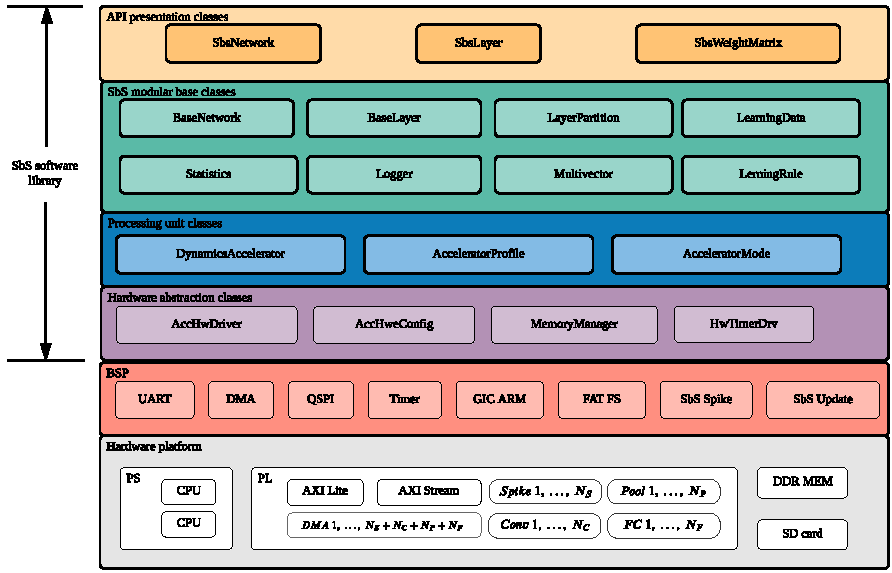
\includegraphics[width=0.5\textwidth]{../figures/sbs_software_component.pdf}
	\caption{System-level overview of the software architecture.}
	\label{fig:sw_stack}
\end{figure}

\subsection{Hardware architecture} \label{Hardware_architecture}
As a hardware/software co-design, the system architecture is an embedded CPU+FPGA-based platform, where the acceleration of SbS network computation is based on asynchronous\footnote{The system is synchronous at the circuit level, but the execution is asynchronous in terms of jobs.} execution \replaced{in}{of} parallel heterogeneous processing units (PUs): \emph{Spike} (input layer), \emph{Conv} (convolution), \emph{Pool} (pooling), and \emph{FC} (fully connected). \fig{fig:hw_sbs} illustrates the system \replaced{hardware architecture}{overview} as a scalable structure. For hardware configuration, each PU uses AXI-Lite interface; for data transfer, each PU uses AXI-Stream interfaces via Direct Memory Access (DMA) allowing data movement with high transfer rate. Each PU asserts an interrupt flag once the task or transaction is complete. This interrupt event is handled by the embedded CPU to collect results and start a new transaction.

The hardware architecture can resize its resource utilization by changing the number of PUs instances, this provides a good trade-off between area and throughput. The dedicated PUs for \emph{Conv}, and \emph{FC} implement the proposed dot-product approximation as a system component. The PUs are written in C using Vivado HLS (High-Level Synthesis) tool. In this publication, we illustrate the integration of the approximate dot-product component on the \emph{Conv} processing unit.

\begin{figure}[t!]
	\centering
	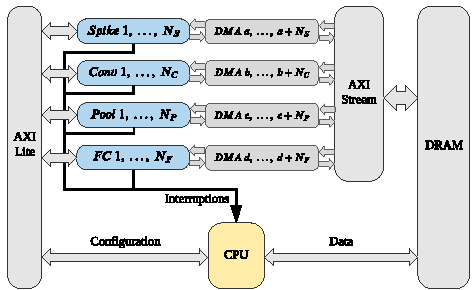
\includegraphics[width=0.5\textwidth]{../figures/sbs_hw.pdf}
	\caption{System-level hardware architecture with scalable number of heterogeneous PUs: \emph{Spike}, \emph{Conv}, \emph{Pool}, and \emph{FC}}
	\label{fig:hw_sbs}
\end{figure}

\subsection{Conv processing unit}
This hardware module computes the IP dynamics defined by \equ{eq:sbs_update} and offers two modes of operation: \emph{configuration} and \emph{computation}.

\subsubsection{Configuration mode}
In this mode of operation, the PU receives and stores in on-chip memory (BRAM) the parameters to compute the IP dynamics: $\epsilon$ as the epsilon, $N$ as the length of $\vec{h}_\mu\in\mathbb{R}^{N}$, $K\in\mathbb{N}$ as the size of the convolution kernel, and $H\in\mathbb{N}$ as the number of IPs to process per transaction. $H$ is the number of IPs forming a layer or a partition.

Additionally, the processing unit also stores in on-chip memory (BRAM) the synaptic weight matrix using a number representation with a reduced memory footprint. Fundamentally, the synaptic weight matrix is defined by $W\in\mathbb{R}^{K\times K\times M\times N}$ with $0\le W(s_t|j)\le1$ and $\sum_{j=0}^{N-1}W(s_t|j)=1$ \cite{rotermund2019Backpropagation}. Hence, $W$ employs only positive normalized real numbers. Therefore, $W$ is deployed using a reduced floating-point or logarithmic representation as follows:

\begin{itemize}
	\item{Custom floating-point representation}.
	In this case, $W$ is deployed with a reduced floating-point representation using the user defined bit width for the exponent and for the mantissa. For example, 4-bit exponent, 1-bit mantissa; as a result: 5-bit custom floating-point.
	\item{Logarithmic representation}.
	In this case, the synaptic weight matrix is $W\in\mathbb{N}^{K\times K\times M\times N}$ with positive natural numbers. Since $0\le W(s_t|j)\le1$ and $\sum_{j=0}^{N-1}W(s_t|j)=1$, $W$ has only negative values in the logarithmic domain. Hence, the sign bit is omitted, and the values are represented in its positive form. Therefore, $W$ is deployed with a representation using the necessary bit width for the exponent according to the given application. For example, 4-bit exponent.
\end{itemize}

In order to deploy different SbS network models, the \emph{Conv} processing units can be set with different synaptic weight matrices and parameters as required through the embedded software.

\subsubsection{Computation mode}
In this mode of operation, the PU executes a transaction to process a group of IPs using the previously given parameters and synaptic weight matrix. This process operates in six stages as shown in \fig{fig:hw_conv}. In the first two stages, the PU receives $\vec{h}_\mu\in\mathbb{R}^{N}$, then the PU calculates the emitted spike, and stores it in $S^{new}\in\mathbb{N}^{H}$ (output spike vector). From the third to the fifth stage, the PU receives $S_t\in\mathbb{N}^{K\times K}$ (input spike matrix), then it computes the update dynamics, and then it dispatches $\vec{h}_\mu^{new}\in\mathbb{R}^{N}$ (updated IP). This process repeats for $H$ number of loops (for each IP of the layer or partition). Finally, the $S^{new}$ is dispatched.

The computation of the update dynamics (see \fig{fig:hw_conv}(d)) operates in two modular stages: \emph{dot-product} and \emph{neuron update}. First, the \emph{dot-product} module calculates the sum of pairwise products of $\vec{h}_{\mu}$ and $\vec{W}(s_t)$, while storing each pairwise product as intermediate results. Subsequently, the \emph{neuron update} module calculates \equ{eq:sbs_update} reusing previous results and parameters.


The computation of the dot-product of \equ{eq:sbs_update} represents a considerable computational cost using standard floating-point in non-quantized network models. Fortunately, the pair product of $h_{\mu}(j)$ and $W(s_t|j)$ was defined by us as an approximable factor in the dot-product of \equ{eq:sbs_update}. In the following section, we focus on an optimized dot-product hardware design based on approximate computing.


\begin{figure}[t!]
	\centering
	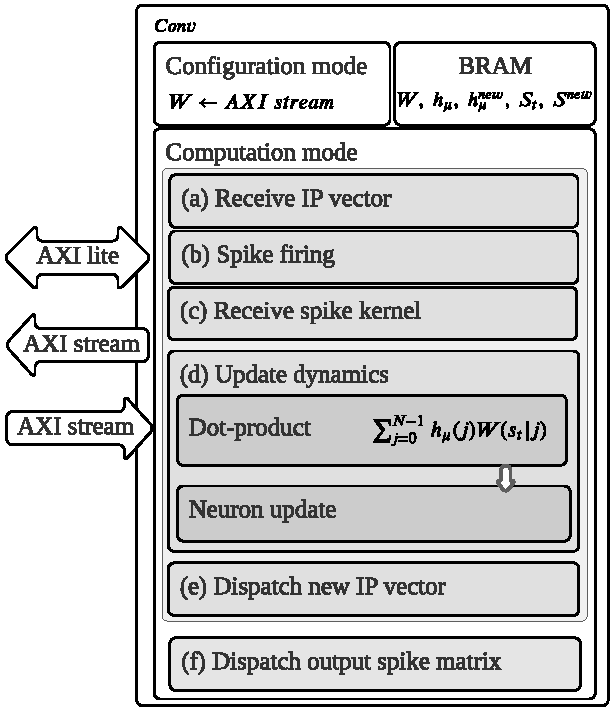
\includegraphics[width=0.5\textwidth]{../figures/sbs_conv.pdf}
	\caption{The \emph{Conv} processing unit and its six stages: (a) receive IP vector, (b) spike firing, (c) receive spike kernel, (d) update dynamics, (e) dispatch new IP vector, (f) dispatch output spike matrix.}
	\label{fig:hw_conv}
\end{figure}

\subsection{dot-product hardware module}
This dot-product hardware module is part of an application-specific architecture optimized to approximate the dot-product of arbitrary length, see \equ{eq:dot_product}. For quality configurability, we parameterized the mantissa bit-width of $\vec{W}(s_t)$, which provides a tunable trade-off between resource utilization and QoR. Since the lower-order bits have smaller significance than the higher-order bits, removing them may have only a minor impact on QoR. We designate this as hybrid custom floating-point approximation.

\begin{eqnarray} \label{eq:dot_product}
r_{\mu}\left(s_t\right)=\sum_{j=0}^{N-1}h_{\mu}(j)W(s_t|j)
\end{eqnarray}

Further on, we remove the mantissa bits completely in order to use only the exponent of a floating-point representation. Hence, the worst-case quality and yet the most efficient configuration becomes a logarithmic representation. Consequently, this configuration leads to advantageous architectural optimizations using only adders and barrel shifters for dot-product approximation in hardware. We designate this as hybrid logarithmic approximation.

In this section, we will present three pipelined hardware modules with standard floating-point computation, hybrid custom floating-point approximation, and hybrid logarithmic approximation.

\subsubsection{Dot-product with standard floating-point computation}
 The hardware module to calculate the dot-product with standard floating-point computation is shown in \fig{fig:dot_product_float}. This diagram presents the hardware blocks and their clock cycle schedule. This module loads both $h_\mu(j)$ and $W(s|j)$ from BRAM, then the PU executes the pairwise product (\fig{fig:dot_product_float}(c)) and accumulation (\fig{fig:dot_product_float}(d)). The intermediate results of $h_\mu(j) W(s_t|j)$ are stored in BRAM for reuse in the neuron update. The latency in clock cycles of this hardware module is defined by \equ{eq:dot_standard_float_latency}, where $N$ is the dot-product length. This latency equation is obtained from the general pipelined hardware latency formula: $L=\left(N-1\right)II+IL$, where $II$ is the initiation interval (\fig{fig:dot_product_float}(a)), and $IL$ is the iteration latency (\fig{fig:dot_product_float}(b)). Both $II$ and $IL$ are obtained from the high-level synthesis analysis. The equation for the latency with standard 32-bit floating-point is:
 \begin{eqnarray} \label{eq:dot_standard_float_latency}
 L_{f32}=10N+9
 \end{eqnarray}
 
In this design, the high level synthesis tool infers computational blocks with considerable latency cost for standard floating-point. In the case of floating-point multiplication (\fig{fig:dot_product_float}(c)), the synthesis infers a hardware block with a latency cost of 5 clock cycles. Theoretically, this block would handle exponents addition, mantissas multiplication, and mantissa correction if needed. Moreover, in the case of floating-point addition (\fig{fig:dot_product_float}(d)), the synthesis infers a hardware block with a latency cost of 9 clock cycles. Seemingly, this block would handle mantissas alignment, addition, and correction if needed. Therefore, the use of standard floating-point in high-level synthesis results in high computational cost, which represents unnecessary overhead in error-tolerant applications.


\begin{figure}[t!]
	\centering
	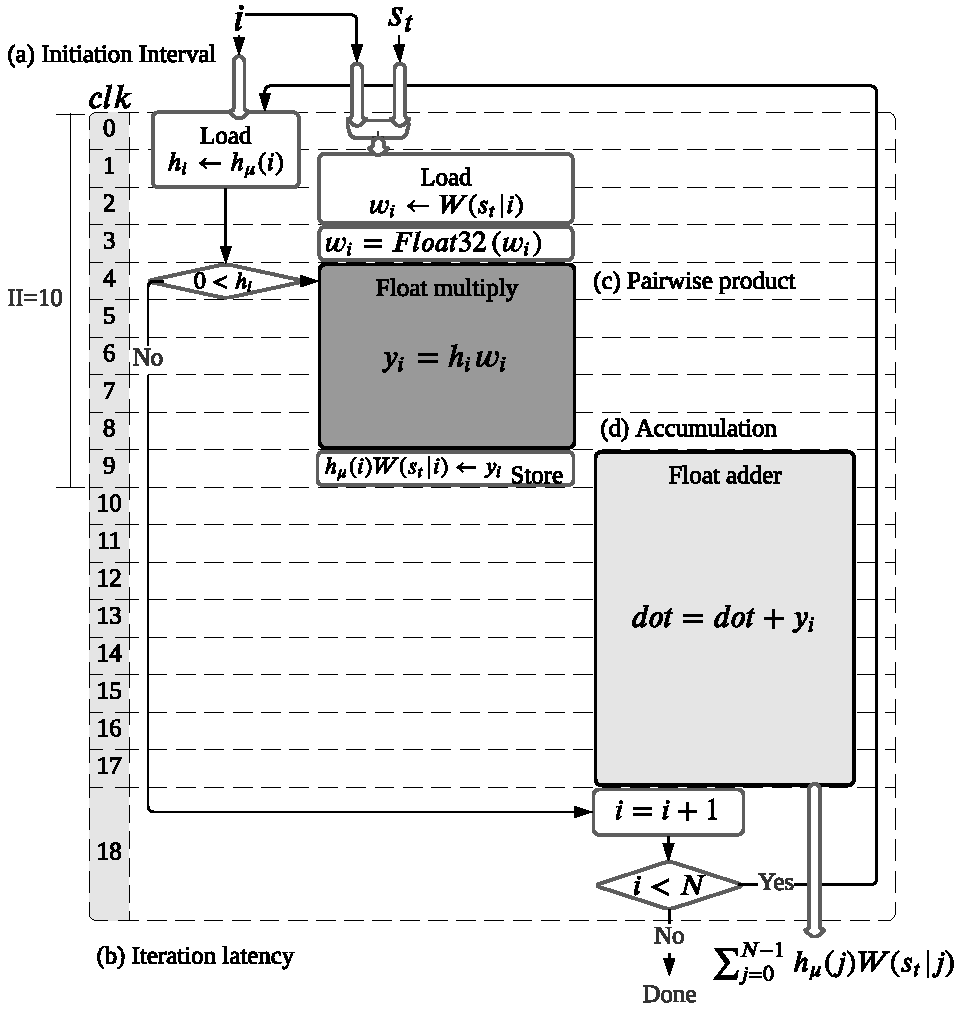
\includegraphics[width=0.5\textwidth]{../figures/dot_product_float.pdf}
	\caption{Dot-product hardware module with standard floating-point computation, (a) exhibits the initiation interval of 10 clock cycles, (b) presents the iteration latency of 19 clock cycles, (c) shows the pairwise product block in dark-gray, and (d) illustrates the accumulation block in light-gray.}
	\label{fig:dot_product_float}
\end{figure}

\subsubsection{Dot-product with hybrid custom floating-point and logarithmic approximation}
 The hardware module to calculate dot-product with hybrid custom floating-point approximation is shown in \fig{fig:dot_product_custom}. In this design, $h_\mu(j)$ uses standard 32-bit floating-point number representation, and $W(s|j)$ uses a positive reduced custom floating-point number representation, where the mantissa bit width is the quality configurability knob. This parameter is tuned by the designer to trade-off between QoR and resource utilization, thus, energy consumption.
 
 As the most efficient setup and yet the worst-case quality configuration, by completely truncating the mantissa of $W(s|j)$ leads to a slightly different hardware architecture using only adders and shifters, which computes the dot-product with hybrid logarithmic approximation. This is shown in \fig{fig:dot_product_log}.
 
Additionally, the exponent bit width of $W(s|j)$ is a design parameter for efficient resource utilization and it is defined based on the application or deployment needs.
 
 The hybrid custom floating-point and logarithmic approximation designs work in three phases: \emph{Computation}, \emph{Threshold-test}, and \emph{Result normalization}.
 
 \begin{itemize}
 	\item{Phase I, \emph{Computation}}: 
 	\\This phase approximates the magnitude of the dot-product in a denormalized representation. This is calculated in two iterative steps over each vector element: \emph{pairwise product} and \emph{accumulation}, where \emph{pairwise product} is executed either in hybrid custom floating-point or hybrid logarithmic approximation described below.
 	 \begin{itemize}[label={--}]
 	 	\item{Pairwise product}.
 	 	\begin{itemize} [label={--}]
	 		\item{Hybrid custom floating-point approximation}.
	 	 	As shown in \fig{fig:dot_product_custom}(c) in dark-gray, the pairwise product is approximated by adding exponents and multiplying mantissas of both $W(s|i)$ and $h_\mu(i)$. If the mantissa multiplication results in an overflow, then it is corrected by increasing the  exponent and shifting the resulting mantissa by one position to the right. Then we get $h_\mu(j) W(s_t|j)$ as an intermediate result which is stored for future reuse in the neuron update calculation. In this design the pairwise product has a latency of 5 clock cycles.
	 	 	\item{Hybrid logarithmic approximation}.
	 	 	As shown in \fig{fig:dot_product_log}(c) in dark-gray, the pairwise product is approximated by adding $W(s|i)$ to the exponent of $h_\mu(i)$, since $W(s|j)$ values are represented in the logarithmic domain and $h_\mu(j)$ in standard floating-point. In this design the pairwise product has a latency of one clock cycle.
 	 	\end{itemize}
 		\item{Accumulation}. As shown in both \fig{fig:dot_product_custom}(d) and \fig{fig:dot_product_log}(d) in light-gray, first, it is obtained the denormalized representation of $h_\mu(j) W(s_t|j)$ by shifting its mantissa using its exponent as shifting parameter (barrel shifter). Then, this denormalized representation is accumulated to obtain the approximated magnitude of the dot-product.
 	 \end{itemize}
 	The process of pairwise product and accumulation iterates over each element of the vectors. The computation latency is given by \equ{eq:dot_standard_custom_float_latency} for hybrid custom floating-point, and \equ{eq:dot_log_latency} for hybrid logarithmic, where $N$ is the length of the vectors. Both pipelined hardware modules have the same throughput, since both have two clock cycles as initiation interval. 	
 	\begin{eqnarray} \label{eq:dot_standard_custom_float_latency}
 	L_{custom}=2N+11
 	\end{eqnarray} 	
	\begin{eqnarray} \label{eq:dot_log_latency}
 	L_{log}=2N+7
 	\end{eqnarray}
 	
 	\item{Phase II, \emph{Threshold-test}}: \\
	The accumulated denormalized magnitude is tested to be above of a predefined threshold, it must be above zero, since the dot-product is the denominator in \equ{eq:sbs_update}.
 	If passing the threshold, then the next phase is executed. Otherwise the rest of update dynamics is skipped. The threshold-test takes one clock cycle.
 	\item{Phase III, \emph{Result-normalization}}: \\
 	In this phase, the dot-product is normalized to obtain the exponent and mantissa in order to convert it to standard floating-point for later use in the neuron update. The normalization is obtained by shifting the approximated dot-product magnitude in a loop until it is in the form of a normalized mantissa where the iteration count represents the exponent of the dot-product. Each iteration takes one clock cycle.
 	
 \end{itemize}


The total latency of the hardware module with hybrid custom floating-point and hybrid logarithmic approximation is the accumulated latency of the three phases.

The proposed architectures with approximation approach exceeds the performance of the design with standard floating-point. This performance enhancement is achieved by decomposing the floating-point computation into an advantageous handling of exponent and mantissa using intermediate accumulation in a denormalized representation and only one final normalization.

\begin{figure}[t!]
	\centering
	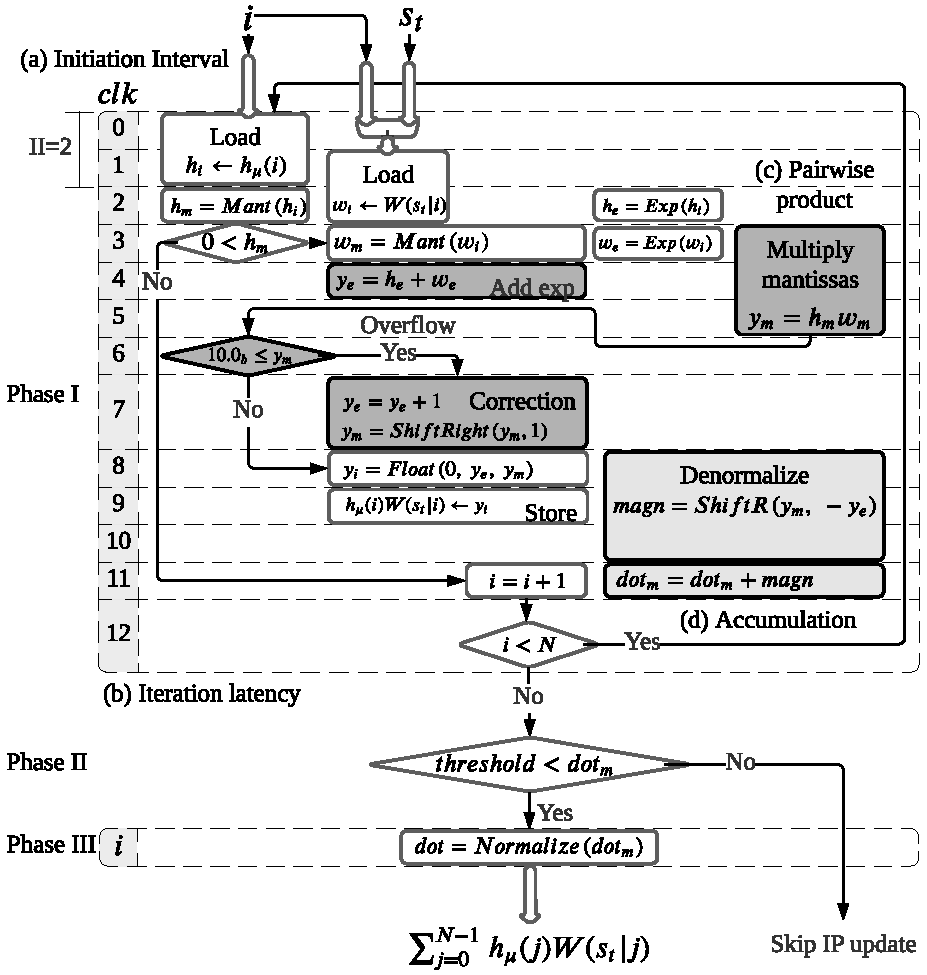
\includegraphics[width=0.5\textwidth]{../figures/dot_product.pdf}
	\caption{Dot-product hardware module with hybrid custom floating-point approximation, (a) exhibits the initiation interval of 2 clock cycles, (b) presents the iteration latency of 13 clock cycles, (c) shows the pairwise product blocks in dark-gray, and (d) illustrates the accumulation blocks in light-gray.}
	\label{fig:dot_product_custom}
\end{figure}

\begin{figure}[t!]
	\centering
	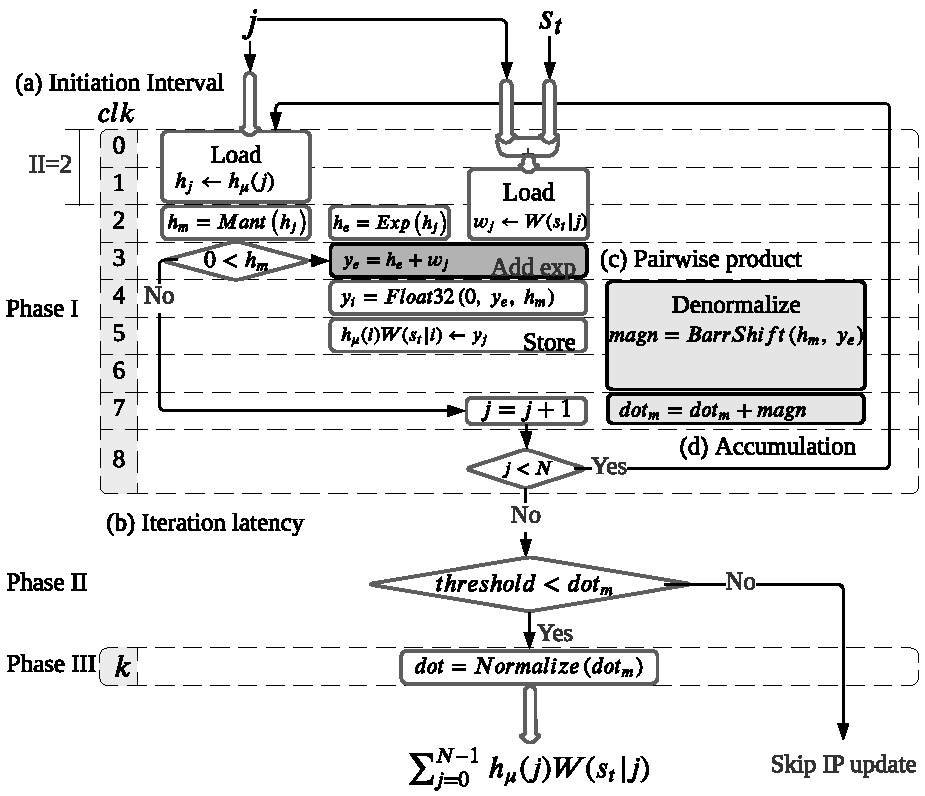
\includegraphics[width=0.5\textwidth]{../figures/dot_product_log.pdf}
	\caption{Dot-product hardware module with hybrid logarithmic approximation, (a) exhibits the initiation interval of 2 clock cycles, (b) presents the iteration latency of 9 clock cycles, (c) shows the pairwise product block in dark-gray, and (d) illustrates the accumulation blocks in light-gray.}
	\label{fig:dot_product_log}
\end{figure}


